% The code is quite messy !!!

\documentclass[tikz,border=10pt]{standalone}

\begin{document}

    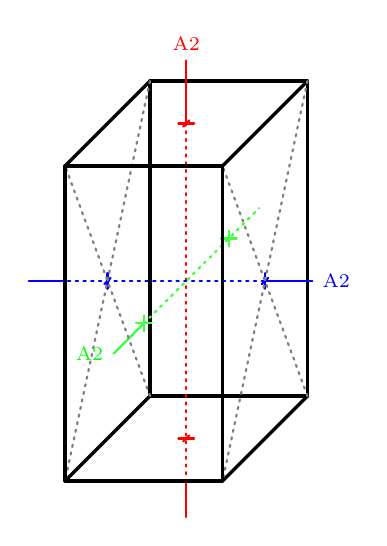
\begin{tikzpicture}[scale=2, line join=round, line cap=round]

        % Définir les sommets d'un cube
        \coordinate (A) at (0, 0, 0);
        \coordinate (B) at (1, 0, 0);
        \coordinate (C) at (1, 2, 0);
        \coordinate (D) at (0, 2, 0);
        \coordinate (E) at (0, 0, 1.4);
        \coordinate (F) at (1, 0, 1.4);
        \coordinate (G) at (1, 2, 1.4);
        \coordinate (H) at (0, 2, 1.4);
            
        \draw[black, very thick] (A) -- (B) -- (C) -- (D) -- cycle; % Face de derriere
        
        % Axe d'ordre 4 (centre de deux faces opposées)
        \draw[red, thick, dotted] (0.5, 2, 0.7) -- (0.5, -0.3, 0.7);
        \draw[red, thick] (0.5, -0.5, 0.7) -- (0.5, -0.28, 0.7);
        \draw[red, thick] (0.5, 2, 0.7) -- (0.5, 2.4, 0.7) node[above, red] {\scriptsize A2};
        \draw[red, thick] (0.5, 0, 0.65) -- (0.5, 0, 0.75); % cross
        \draw[red, thick] (0.45, 0, 0.7) -- (0.55, 0, 0.7); % cross
        \draw[red, thick] (0.5, 2, 0.65) -- (0.5, 2, 0.75); % cross
        \draw[red, thick] (0.45, 2, 0.7) -- (0.55, 2, 0.7); % cross

        % Axe d'ordre 4 (centre de deux faces opposées)
        \draw[blue, thick, dotted] (-0.3, 1, 0.7) -- (1, 1, 0.7);
        \draw[blue, thick] (-0.3, 1, 0.7) -- (-0.5, 1, 0.7);
        \draw[blue, thick] (1, 1, 0.7) -- (1.3, 1, 0.7) node[right, blue] {\scriptsize A2};
        \draw[blue, thick] (0, 1, 0.65) -- (0, 1, 0.75); % cross
        \draw[blue, thick] (0, 1.05, 0.7) -- (0, 0.95, 0.7); % cross
        \draw[blue, thick] (1, 1, 0.65) -- (1, 1, 0.75); % cross
        \draw[blue, thick] (1, 1.05, 0.7) -- (1, 0.95, 0.7); % cross

        % Axe d'ordre 4 (centre de deux faces opposées)
        \draw[green!75, thick, dotted] (0.5, 1, 1.4) -- (0.5, 1, -0.5);
        \draw[green!75, thick] (0.5, 1, 1.4) -- (0.5, 1, 1.9) node[left, green] {\scriptsize A2};
        \draw[green!75, thick] (0.45, 1, 0) -- (0.55, 1, 0); % cross
        \draw[green!75, thick] (0.5, 0.95, 0) -- (0.5, 1.05, 0); % cross
        \draw[green!75, thick] (0.45, 1, 1.4) -- (0.55, 1, 1.4); % cross
        \draw[green!75, thick] (0.5, 0.95, 1.4) -- (0.5, 1.05, 1.4); % cross


        \draw[black, very thick] (A) -- (E); % Arêtes verticales
        \draw[black, very thick] (B) -- (F);
        \draw[black, very thick] (C) -- (G);
        \draw[black, very thick] (D) -- (H);

        % diagonale
        \draw[gray, thick, dotted] (D) -- (E);
        \draw[gray, thick, dotted] (B) -- (G);
        \draw[gray, thick, dotted] (C) -- (F);
        \draw[gray, thick, dotted] (A) -- (H);

        % Tracer les arêtes du cube
        \draw[black, very thick] (E) -- (F) -- (G) -- (H) -- cycle; % Face supérieure

    \end{tikzpicture}

\end{document}